% !TeX encoding = UTF-8
% !TeX spellcheck = pl_PL

% $Id:$

%Author: Wojciech Domski
%Szablon do ząłożeń projektowych, raportu i dokumentacji z steorwników robotów
%Wersja v.1.0.0
%


%% Konfiguracja:
\newcommand{\kurs}{Roboty mobilne}
\newcommand{\formakursu}{Projekt}

%odkomentuj właściwy typ projektu, a pozostałe zostaw zakomentowane
%\newcommand{\doctype}{Za\l{}o\.{z}enia projektowe} %etap I
%\newcommand{\doctype}{Raport} %etap II
\newcommand{\doctype}{Dokumentacja} %etap III

%wpisz nazwę projektu
\newcommand{\projectname}{Linefollower}

%wpisz akronim projektu
\newcommand{\acronim}{LF}

%wpisz Imię i nazwisko oraz numer albumu
\newcommand{\osobaA}{Cyprian \textsc{Hryniuk}, 235512}
%w przypadku projektu jednoosobowego usuń zawartość nowej komendy
\newcommand{\osobaB}{Tomasz \textsc{Mas\l{}o\'n}, 235827}

%wpisz termin w formie, jak poniżej dzień, parzystość, godzina
\newcommand{\termin}{wtTP15}

%wpisz imię i nazwisko prowadzącego
\newcommand{\prowadzacy}{mgr in\.{z}. Micha\l{} \textsc{B\l{}\k{e}dowski}}

\documentclass[10pt, a4paper]{article}

%Preambuła dokumentu

% linki w spisie tresci, bibliografi
\usepackage[bookmarks=true,bookmarksnumbered=false,unicode=true,pdftex=true, colorlinks,filecolor=black,linkcolor=black,urlcolor=black,citecolor=black]{hyperref}

%ustawienie rozmiaru papieru
\usepackage[a4paper, left=2.5cm, right=2.5cm, top=2.5cm, bottom=2.5cm, headsep=1.2cm]{geometry}

%rozmaite ustawienia pozwalające okreslić język

%NALEŻY wybrać jeden z pakietów
%\usepackage{polski} %przydatne podczas składania dokumentów w j. polskim
\usepackage[polish]{babel}  % pakiet lokalizujący dokument w języku polskim
%\usepackage[british]{babel}

\usepackage{indentfirst}	% polski styl pisania (np. rozpoczecie pierwszego akapitu
% pod nazwa rozdzialu od wciecia)
%\usepackage[OT4]{fontenc}
\usepackage[utf8]{inputenc} % w miejsce utf8 można wpisać latin2 bądź cp1250,
% w zależności od tego w jaki sposób kodowane są 
% polskie znaki diakrytyczne przy wprowadzaniu 
% z klawiatury.
%kodowanie znaków, zależne od systemu
\usepackage[T1]{fontenc} %poprawne składanie polskich czcionek

%OPEROWANIE NA OBRAZACH
\usepackage{graphicx}       % pakiet graficzny, umożliwiający m.in.
% import grafik w formacie eps
%\usepackage{epstopdf}		% pozwala na importowanie grafik w formacie eps
% przy użyciu pdflatex
\usepackage[update,prepend]{epstopdf}
\usepackage{rotating}       % pakiet umożliwiający obracanie rysunków
\usepackage{subfigure}      % pakiet umożliwiający tworzenie podrysunków
\usepackage{epic}           % pakiet umożliwiający rysowanie w środowisku latex
\usepackage{psfrag}         % pakiet umożliwiający podmianę łańcuchów znaków 
% w plikach eps
%\usepackage{curves}         % pakiet do wykreslania krzywych

%pakiety dodające dużo dodatkowych poleceń matematycznych
\usepackage{amsfonts}       % pakiet z rozmaitymi czcionkami matematycznymi
%\usepackage{amssymb}        % pakiet z rozmaitymi symbolami matematycznymi
\usepackage{amsmath}        % pakiet z rozmaitymi środowiskami matematycznymi

\usepackage{fp}             % pakiet z funkcjami operujacymi 
% na liczbach zmiennoprzecinkowych
\usepackage{calc}           % pakiet umożliwiający operacje arytmetyczne
% na tzw. licznikach (liczbach całkowitych)
\usepackage{leftidx}		% indeksy górne i dolne po lewej stronie

%definicje matematyczne
\providecommand{\abs}[1]{\lvert#1\rvert}
\providecommand{\norm}[1]{\lVert#1\rVert}

%pakiety wspomagające i poprawiające składanie tabel
\usepackage{supertabular}
\usepackage{array}
\usepackage{tabularx}
\usepackage{hhline}
\usepackage{longtable}		% wsparcie dla dlugich tabel
\usepackage{multicol}		% podzial strony na wiele kolumn

%pakiet do BibTex
\usepackage{cite}

\usepackage{url} %pakiet pozawalający na dodawanie adresów url w bibliografi

%pakiet wypisujący na marginesie etykiety równań i rysunków zdefiniowanych przez \label{}, chcąc wygenerować finalną wersję dokumentu wystarczy usunąć poniższą linię
%\usepackage{showlabels}

\usepackage{float}			% lepsza obsluga mechanizmow obiektow plywajacych
% wymuszenie wstawienia np. tabeli, obrazka w danym miejscu przez [H]

\usepackage{listings}       % pakiet dedykowany zrodlom programow
\usepackage{color}


\definecolor{dkgreen}{rgb}{0,0.6,0}
\definecolor{gray}{rgb}{0.5,0.5,0.5}
\definecolor{mauve}{rgb}{0.58,0,0.82}

\lstset{ %
	language=C,                % the language of the code
	basicstyle=\small,           % the size of the fonts that are used for the code
	numbers=left,                   % where to put the line-numbers
	numberstyle=\footnotesize\color{gray},  % the style that is used for the line-numbers
	stepnumber=1,                   % the step between two line-numbers. If it's 1, each line 
	% will be numbered
	numbersep=5pt,                  % how far the line-numbers are from the code
	backgroundcolor=\color{white},      % choose the background color. You must add \usepackage{color}
	showspaces=false,               % show spaces adding particular underscores
	showstringspaces=false,         % underline spaces within strings
	showtabs=false,                 % show tabs within strings adding particular underscores
	%frame=single,                   % adds a frame around the code
	rulecolor=\color{black},        % if not set, the frame-color may be changed on line-breaks within not-black text (e.g. comments (green here))
	tabsize=2,                      % sets default tabsize to 2 spaces
	captionpos=b,                   % sets the caption-position to bottom
	breaklines=true,                % sets automatic line breaking
	breakatwhitespace=false,        % sets if automatic breaks should only happen at whitespace
	%title=\lstname,                   % show the filename of files included with \lstinputlisting;
	% also try caption instead of title
	keywordstyle=\color{blue},          % keyword style
	commentstyle=\color{dkgreen},       % comment style
	stringstyle=\color{mauve},         % string literal style
	escapeinside={\%*}{*)},            % if you want to add LaTeX within your code
	morekeywords={*,...},              % if you want to add more keywords to the set
	deletekeywords={...}              % if you want to delete keywords from the given language
}

%polish signs in lst code
\lstset{literate=%
	{ą}{{\k{a}}}1
	{ć}{{\'c}}1
	{ę}{{\k{e}}}1
	{ł}{{\l}}1
	{ń}{{\'n}}1
	{ó}{{\'o}}1
	{ś}{{\'s}}1
	{ż}{{\.z}}1
	{ź}{{\'z}}1
	{Ą}{{\k{A}}}1
	{Ć}{{\'C}}1
	{Ę}{{\k{E}}}1
	{Ł}{{\L}}1
	{Ń}{{\'N}}1
	{Ó}{{\'O}}1
	{Ś}{{\'S}}1
	{Ż}{{\.Z}}1
	{Ź}{{\'Z}}1
}

\usepackage{verbatim}       % pakiet dedykowany rozmaitym wydrukom tekstowym
\usepackage{ifthen}         % pakiet umożliwiający tworzenie prostych programów
% (m.in. zawiera instrukcje powtórzeniowe 
% i warunkowe)
\usepackage{upquote}		%normal quotations marks ' and `

% deklaracje wymagane przez pakiet theorem automatycznie ladowany w przypadku
% klasy dokumentu article
%
\newtheorem{Dn}{Definicja}[section]     % deklaracja srodowiska definicja
\newtheorem{La}[Dn]{Lemat}                % deklaracja srodowiska lemat
\newtheorem{Tm}[Dn]{Twierdzenie}          % deklaracja srodowiska twierdzenie
\newtheorem{Rk}[Dn]{Spostrze{\.z}enie}  % deklaracja srodowiska spostrzezenie
\newtheorem{Am}[Dn]{Algorytm}           % deklaracja srodowiska algorytm
\newtheorem{As}[Dn]{Za{\l}o{\.z}enie}   % deklaracja srodowiska zalozenie
\newtheorem{Pn}[Dn]{Propozycja}           % deklaracja srodowiska propozycja
\newtheorem{Py}[Dn]{W{\l}asno{\'s}{\'c}}  % deklaracja srodowiska wlasnosc
\newtheorem{Cy}[Dn]{Wniosek}              % deklaracja srodowiska wniosek
\newtheorem{Ee}[Dn]{Przyk{\l}ad}        % deklaracja srodowiska przyklad
\newtheorem{Ex}{{\'C}wiczenie}          % deklaracja srodowiska cwiczenie

%helps to specify width of a column in table
%\begin{tabular}{|C{1cm}|c|c|c|c|c|c|c|c|c|c|}
%first column will have widht of 1cm
\newcolumntype{L}[1]{>{\raggedright\let\newline\\\arraybackslash\hspace{0pt}}m{#1}}
\newcolumntype{C}[1]{>{\centering\let\newline\\\arraybackslash\hspace{0pt}}m{#1}}
\newcolumntype{R}[1]{>{\raggedleft\let\newline\\\arraybackslash\hspace{0pt}}m{#1}}

\sloppy			%zawija bardzo długie linie

%\pagenumbering{gobble}% Remove page numbers (and reset to 1)
\graphicspath{{./img/}}

\begin{document}

\def\tablename{Tabela}	%zmienienie nazwy tabel z Tablica na Tabela

\begin{titlepage}
	\begin{center}
		\textsc{\LARGE \formakursu}\\[1cm]		
		\textsc{\Large \kurs}\\[0.5cm]		
		\rule{\textwidth}{0.08cm}\\[0.4cm]
		{\huge \bfseries \doctype}\\[1cm]
		{\huge \bfseries \projectname}\\[0.5cm]
		{\huge \bfseries \acronim}\\[0.4cm]
		\rule{\textwidth}{0.08cm}\\[1cm]
		
		\begin{flushright} \large
		\emph{Skład grupy:}\\
		\osobaA\\
		\osobaB\\[0.4cm]
		
		\emph{Termin: }\termin\\[0.4cm]

		\emph{Prowadzący:} \\
		\prowadzacy \\
		
		\end{flushright}
		
		\vfill
		
		{\large \today}
	\end{center}	
\end{titlepage}

\newpage
\tableofcontents
\newpage

%Obecne we wszystkich dokumentach
\section{Opis projektu}
\label{sec:OpisProjektu}
Projekt ma na celu stworzenie linefollowera - robota klasy k(2,0) poruszającego się po wyznaczonej linii. Prace projektowe zawierać w sobie będą projekt i wykonanie układu mechanicznego i układu elektronicznego, wytworzenie oprogramowania oraz montaż robota.

Robot będzie wykrywać linię za pomocą zestawu czujników odbiciowych. Sygnał z czujników przekazywany będzie do mikrokontrolera, który w oparciu o dane z czujników, będzie sterował silnikami prądu stałego pełniącymi rolę napędową kół. Całość zasilana będzie akumulatorem litowo-polimerowym.

Sterowanie silnikami odbywać się będzie przy pomocy mostków-H. Algorytm sterujący wykorzystywać będzie regulator PD (w którym błąd będzie określany na podstawie sygnałów z czujników i odzwierciedlać będzie odbieganie toru jazdy od aktualnego kierunku, w którym linefollower się porusza), aby płynnie reagować na zmiany toru jazdy.
%\begin{figure}[H]
%	\centering
%	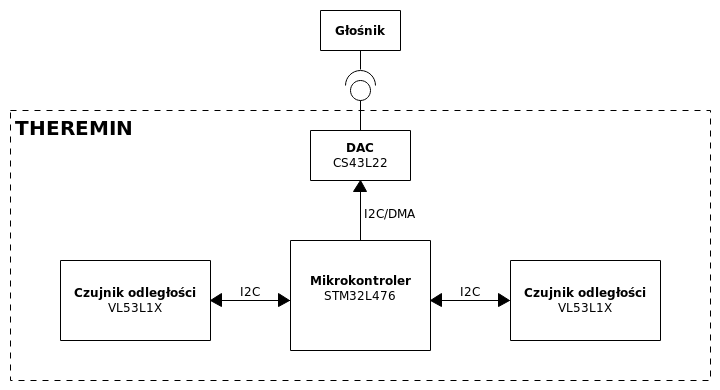
\includegraphics[width=0.8\textwidth]{architektura.png}
%	\caption{Architektura systemu}
%	\label{fig:Architektura}
%\end{figure}


%\section{Założenia projektowe}
%?????

 
%Obecne we wszystkich dokumentach
\section{Konfiguracja mikrokontrolera}

\begin{figure}[H]
	\centering
	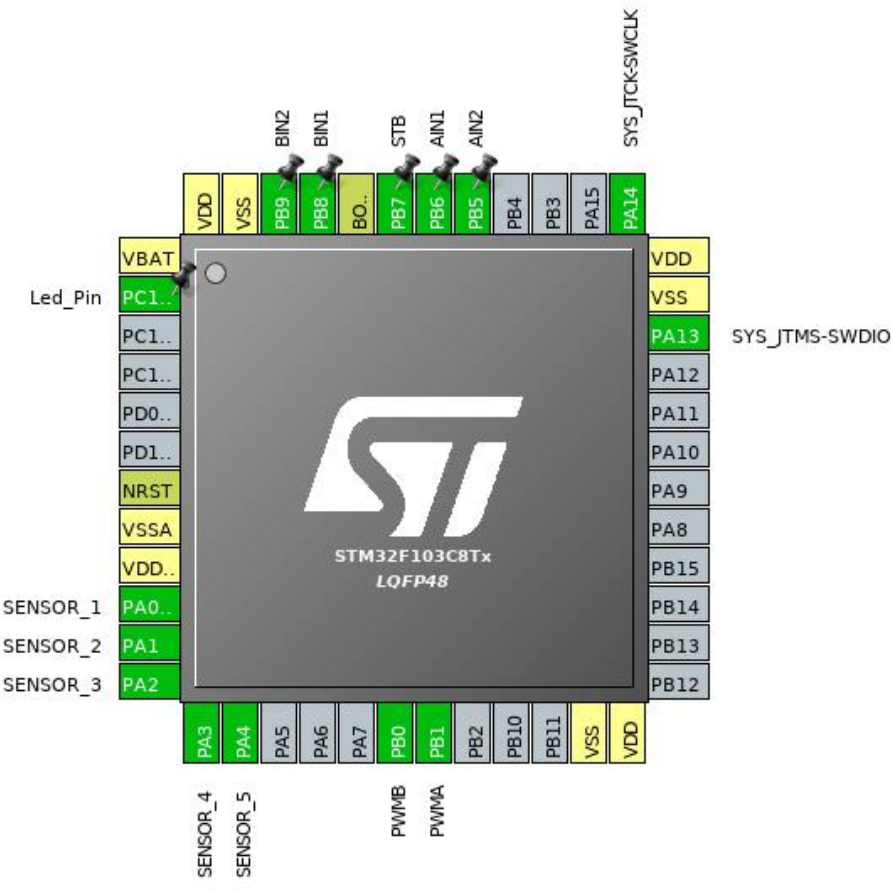
\includegraphics[width=0.8\textwidth]{konfiguracja_mcu.png}
	\caption{Konfiguracja wyjść mikrokontrolera w programie STM32CubeMX}
	\label{fig:KonfiguracjaMikrokontrolera}
\end{figure}

\newpage
\begin{figure}[H]
	\centering
	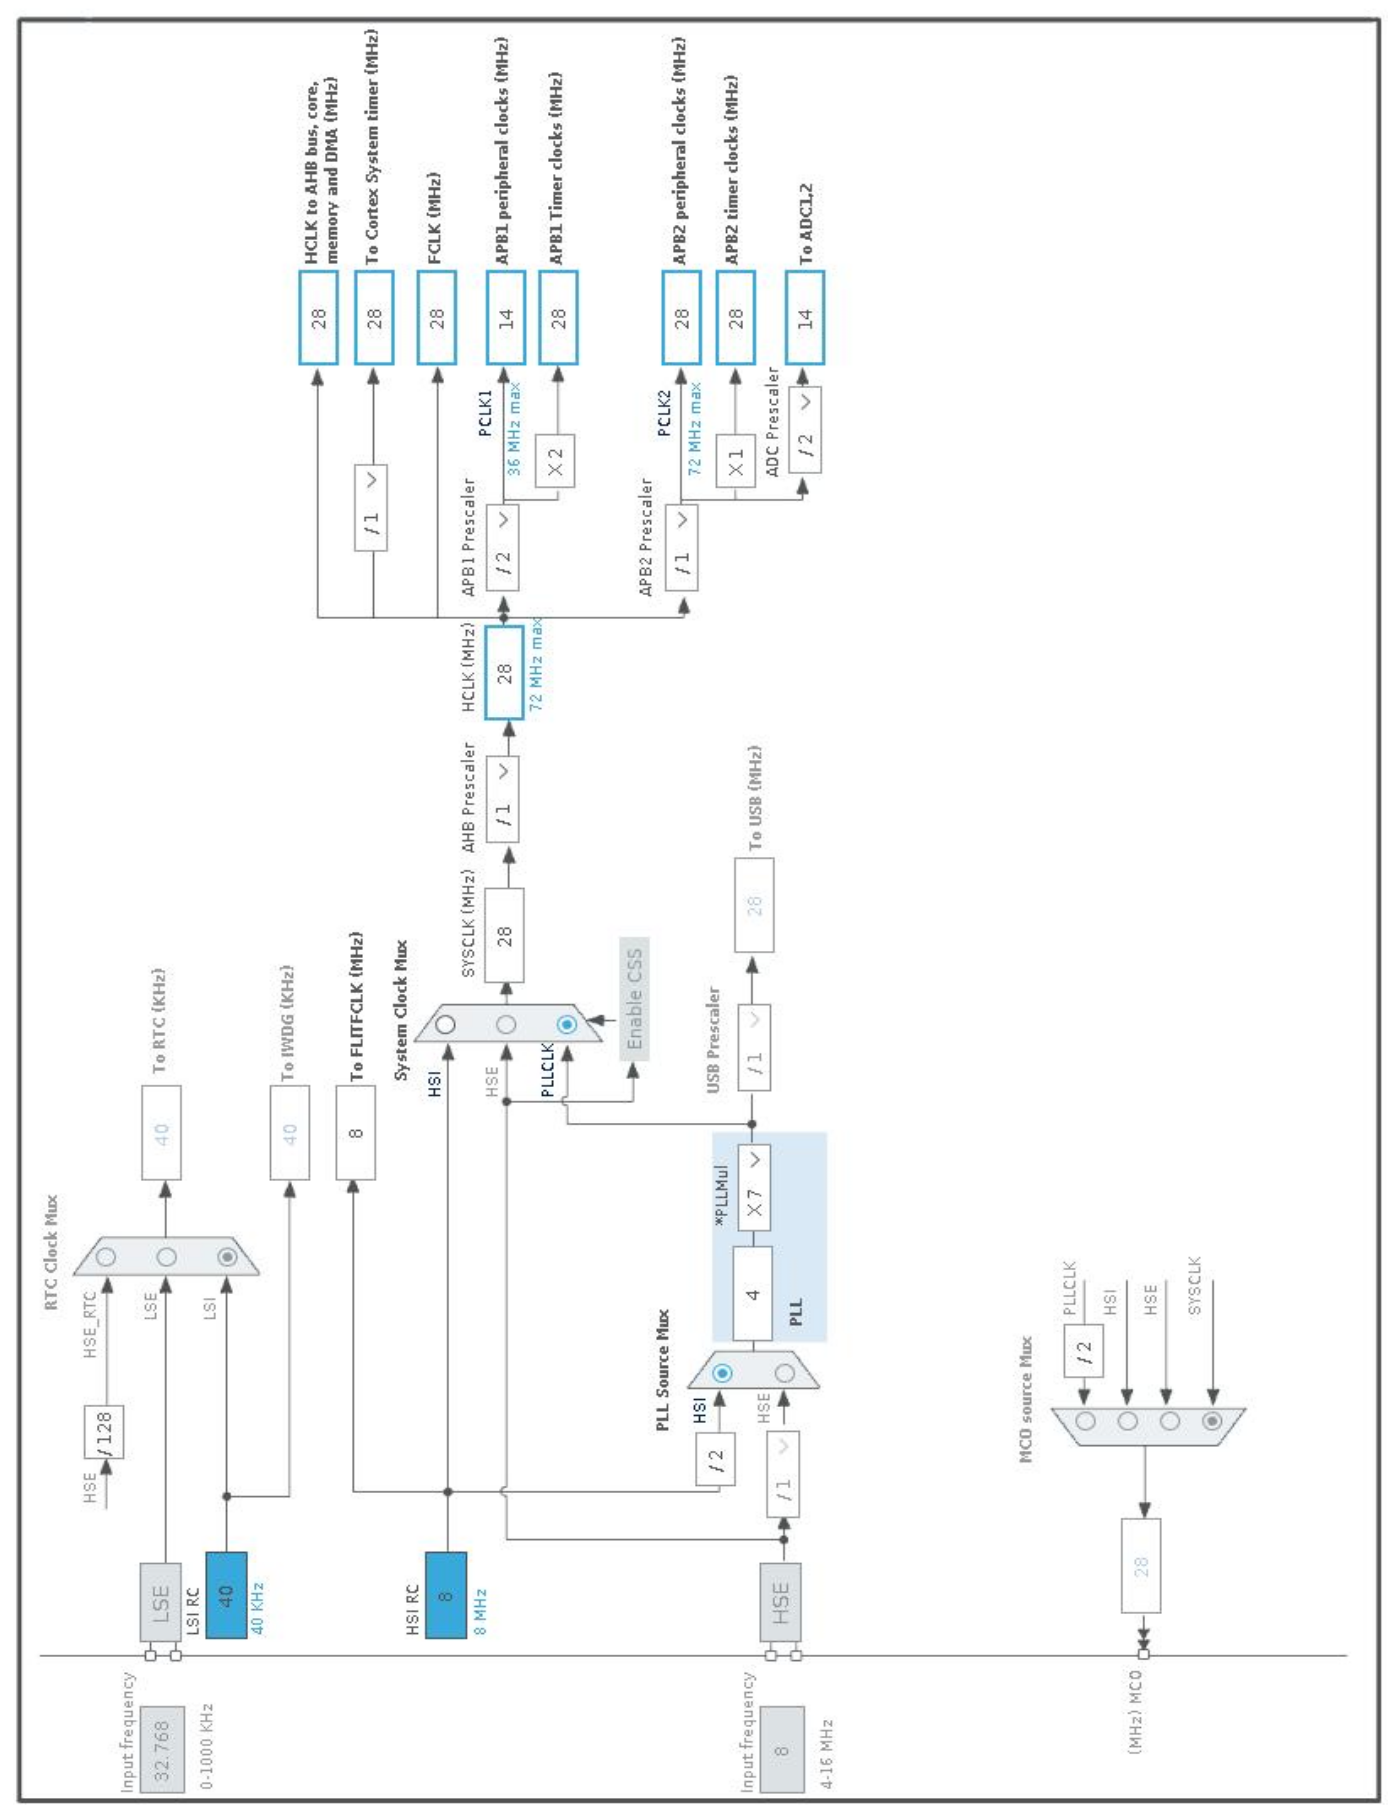
\includegraphics[width=\textwidth]{konfiguracja_clk.png}
	\caption{Konfiguracja zegarów mikrokontrolera}
	\label{fig:KonfiguracjaZegara}
\end{figure}

%Obecne we wszystkich dokumentach

\subsection{Konfiguracja pinów}
\noindent Poniżej zawarto konfiguracje pinów mikrokontrolera wraz z etykietami i trybem pracy.
\begin{table}[H]
	\centering
	\begin{tabular}{|l|l|l|l|}
		\hline
		Numer pinu	&	PIN & Tryb pracy & Funkcja/etykieta\\
		\hline
		2&	PC13 & GPIO\_Output &	Led\_Pin	\\
		10&	PA0 & ADC1\_IN0 &	SENSOR\_1	\\
		11&	PA1 & ADC1\_IN1 &	SENSOR\_2	\\
		12&	PA2 & ADC1\_IN2 &	SENSOR\_3\\
		13&	PA3 &	ADC1\_IN3&	SENSOR\_4 \\
		14&	PA4 &	ADC1\_IN4&	SENSOR\_5\\
		18&	PB0 &	TIM3\_CH3&	PWMB\\
		19&	PB1 &	TIM3\_CH3&	PWMA\\
		34&	PA13 &	SYS\_JTMS-SWDIO&	SYS\_JTMS-SWDIO\\
		37&	PA14 &	SYS\_JTCK-SWCLK&	SYS\_JTCK-SWCLK\\
		41&	PB5 &	GPIO\_Output&	AIN2\\
		42&	PB6 &	GPIO\_Output&	AIN1\\
		43&	PB7 &	GPIO\_Output&	STB\\
		45&	PB8 &	GPIO\_Output&	BIN1\\
		46&	PB9 &	GPIO\_Output&	BIN2\\
		\hline
	\end{tabular}
	\caption{Konfiguracja pinów mikrokontrolera}
	\label{tab:KonfiguracjaPinów}	
\end{table}

%Obecne we wszystkich dokumentach
\subsection{TIM3}
\noindent Timer wykorzystywany był do generacji sygnału PWM przekazywanego na sterownik silników. Kanał 3 sterował kołem lewym, a kanał 4 kołem prawym.
\begin{table}[H]
	\centering
	\begin{tabular}{|l|c|} \hline
		\textbf{Parametr} & Wartość \\
		\hline
		\hline  \textbf{Channel3}& PWM Generation CH3\\\hline
		\textbf{Channel4} & PWM Generation CH4\\
		\hline
		\textbf{Prescaler} & 0\\
		\hline	
		\textbf{Counter Period} & 500\\
		\hline	
		\textbf{Trigger Event Selection} & Reset\\
		\hline
	\end{tabular}
	\caption{Konfiguracja peryferium TIM3}
	\label{tab:TIM3}
\end{table}

\subsection{ADC}
\noindent ADC umożliwia odczyt pomiarów dokonywanych przez transoptory odbiciowe. Każdy kanał odpowiada za obsługę jednego czujnika. Odczyt realizowany jest z wykorzystaniem DMA.
\begin{table}[H]
	\centering
	\begin{tabular}{|l|c|} \hline
		\textbf{Parametr} & Wartość \\
		\hline
		\hline  \textbf{Data Alignment}& Right alignment\\\hline
		\textbf{Scan Conversion Mode} & Enabled\\
		\hline
		\textbf{Enable Regular Conversions} & Enable\\
		\hline
		\textbf{Number Of Conversion} & 5\\
		\hline
		\textbf{Rank} & 1..5\\
		\hline
		\textbf{Sampling Time} & 71.5 Cycles\\
		\hline
	\end{tabular}
	\caption{Konfiguracja peryferium ADC}
	\label{tab:ADC}
\end{table}

\subsection{DMA}
\noindent DMA skonfigurowano pod obsługę peryferium ADC. 
\begin{table}[H]
	\centering
	\begin{tabular}{|l|c|} \hline
		\textbf{Parametr} & Wartość \\
		\hline
		\hline  \textbf{DMA request}& ADC1\\\hline
		\textbf{Stream} & DMA1\_Channel1\\
		\hline
		\textbf{Direction} & Peripheral To Memory\\
		\hline
		\textbf{Mode} & Circular\\
		\hline
		\textbf{Peripheral Increment} & Disable\\
		\hline
		\textbf{Memory Increment} & Enable\\
		\hline
		\textbf{Peripheral Data Width} & Word\\
		\hline
		\textbf{Memory Data Width} & Word\\
		\hline
	\end{tabular}
	\caption{Konfiguracja peryferium DMA}
	\label{tab:DAC}
\end{table}

\section{Wykorzystane komponenty}
\subsection{Mikrokontroler - STM32F103C8}
\noindent Tani i popularny mikrokontroler na płytce z oscylatorem i wyprowadzonymi pinami do programowania/debugowania. Znany pod nazwą \textit{Blue pill} z uwagi na kolor soldermaski.

\begin{table}[H]
	\centering
	\begin{tabular}{|l|c|} \hline
		\textbf{Parametr} & Wartość \\
		\hline
		\hline  \textbf{Zegar}& 72MHz\\\hline
		\textbf{RAM} & 20KB\\
		\hline
		\textbf{Pamięć flash} & 64KB/128KB\\
		\hline
	\end{tabular}
	\caption{Podstawowe parametry STM32F103}
	\label{tab:MCU}
\end{table}

\subsection{Mostek H - TB6612FNG}
\noindent Wydajny sterownik silników w małej obudowie SSOP24. Posiada zabezpieczenie przeciwko prądowi zwrotnemu z silników, wbudowany termiczny obwód odcinający, kondensatory filtrujące. Ma do wyboru cztery tryby pracy: swobodne hamowanie, gwałtowne hamowanie, napędzanie kół zgodnie z ruchem wskazówek zegara i przeciwnie do ruchu wskazówek zegara. 

\begin{table}[H]
	\centering
	\begin{tabular}{|l|c|} \hline
		\textbf{Parametr} & Wartość \\
		\hline
		\hline  \textbf{Zasilanie silników (VMOT)}& od 4.5V do 13.5V\\\hline
		\textbf{Zasilanie układu logicznego (VCC)} & od 2.7V do 5.5V\\
		\hline
		\textbf{Maks. prąd wyjściowy (na kanał)} & 3A\\
		\hline
				\textbf{Ciągły prąd wyjściowy (na kanał)} & 1A\\
		\hline
				\textbf{Maksymalna częstotliwość PWM} & 100kHz\\
		\hline
	\end{tabular}
	\caption{Podstawowe parametry TB6612FNG}
	\label{tab:Toshiba}
\end{table}

\subsection{Transoptor odbiciowy - CNY70}
\noindent Czujnik wysyła wiązkę promieniowania przez diodę IR i następnie natężenie światła odbitego za pomocą fototranzystora. Wyjściem czujnika jest napięcie zależne od natężenia światła padającego na tranzystor. Im powierzchnia bardziej odbija światło (jest bardziej jasna) tym wyższe napięcie na wyjściu układu. 

\begin{table}[H]
	\centering
	\begin{tabular}{|l|c|} \hline
		\textbf{Parametr} & Wartość \\
		\hline
		\hline  \textbf{Napięcie zasilania diody}& 5V\\\hline
		\textbf{Maks. prąd diody} & 50mA\\
		\hline
		\textbf{Maks. napięcie kolektor-emiter} & 32V\\
		\hline
		\textbf{Maks. prąd kolektora} & 50mA\\
		\hline
	\end{tabular}
	\caption{Podstawowe parametry CNY70}
	\label{tab:CNY70}
\end{table}

\subsection{Stabilizator - LM7805}
\noindent Stabilizator wykorzystywany do zasilania diody w czujnikach odbiciowych. 

\begin{table}[H]
	\centering
	\begin{tabular}{|l|c|} \hline
		\textbf{Parametr} & Wartość \\
		\hline
		\hline  \textbf{Napięcie wyjściowe ($\pm 2\%$)}& 5V\\\hline
		\textbf{Maks. prąd wyjściowy} & 1.5A\\
		\hline
		\textbf{Maks. napięcie wejściowe} & 35V\\
		\hline
	\end{tabular}
	\caption{Podstawowe parametry LM7805}
	\label{tab:LM7805}
\end{table}

\subsection{Stabilizator - LD1117V33}
\noindent Stabilizator wykorzystywany do zasilania mikrokontrolera oraz układu logicznego sterownika silników.

\begin{table}[H]
	\centering
	\begin{tabular}{|l|c|} \hline
		\textbf{Parametr} & Wartość \\
		\hline
		\hline  \textbf{Napięcie wyjściowe ($\pm 2\%$)}& 3.3V\\\hline
		\textbf{Maks. prąd wyjściowy} & 1.3A\\
		\hline
		\textbf{Maks. napięcie wejściowe} & 15V\\
		\hline
	\end{tabular}
	\caption{Podstawowe parametry LD1117V33}
	\label{tab:LD1117V33}
\end{table}
%Obecne w dokumencie do etapu I
\section{Opis działania urządzenia}
	Na starcie dochodzi do inicjalizacji mikrokontrolera wraz z wszystkimi jego peryferiami. Zasilane są transoptory oraz sterownik silników. Po inicjalizacji sterownik silników przechodzi ze stanu uśpienia w stan gotowości (sygnał wysoki na pin STB). W tym momencie po zarejestrowaniu czarnej linii pod jednym z czujników robot zaczyna za nią podążąć. Jeżeli robot zgubi linie to zostaje zatrzymany swobodnym hamowaniem (PWM = 0\%). 
\begin{figure}[H]
	\centering
	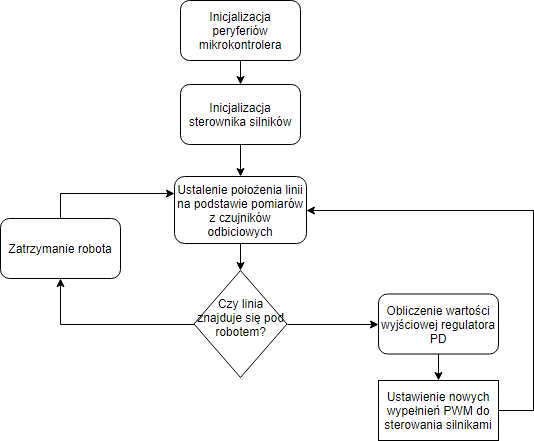
\includegraphics[width=0.9\textwidth]{flowchart.png}
	\caption{Diagram obrazujący działanie urządzenia}
	\label{fig:FlowChart}
\end{figure}
	
\begin{figure}[H]
	\centering
	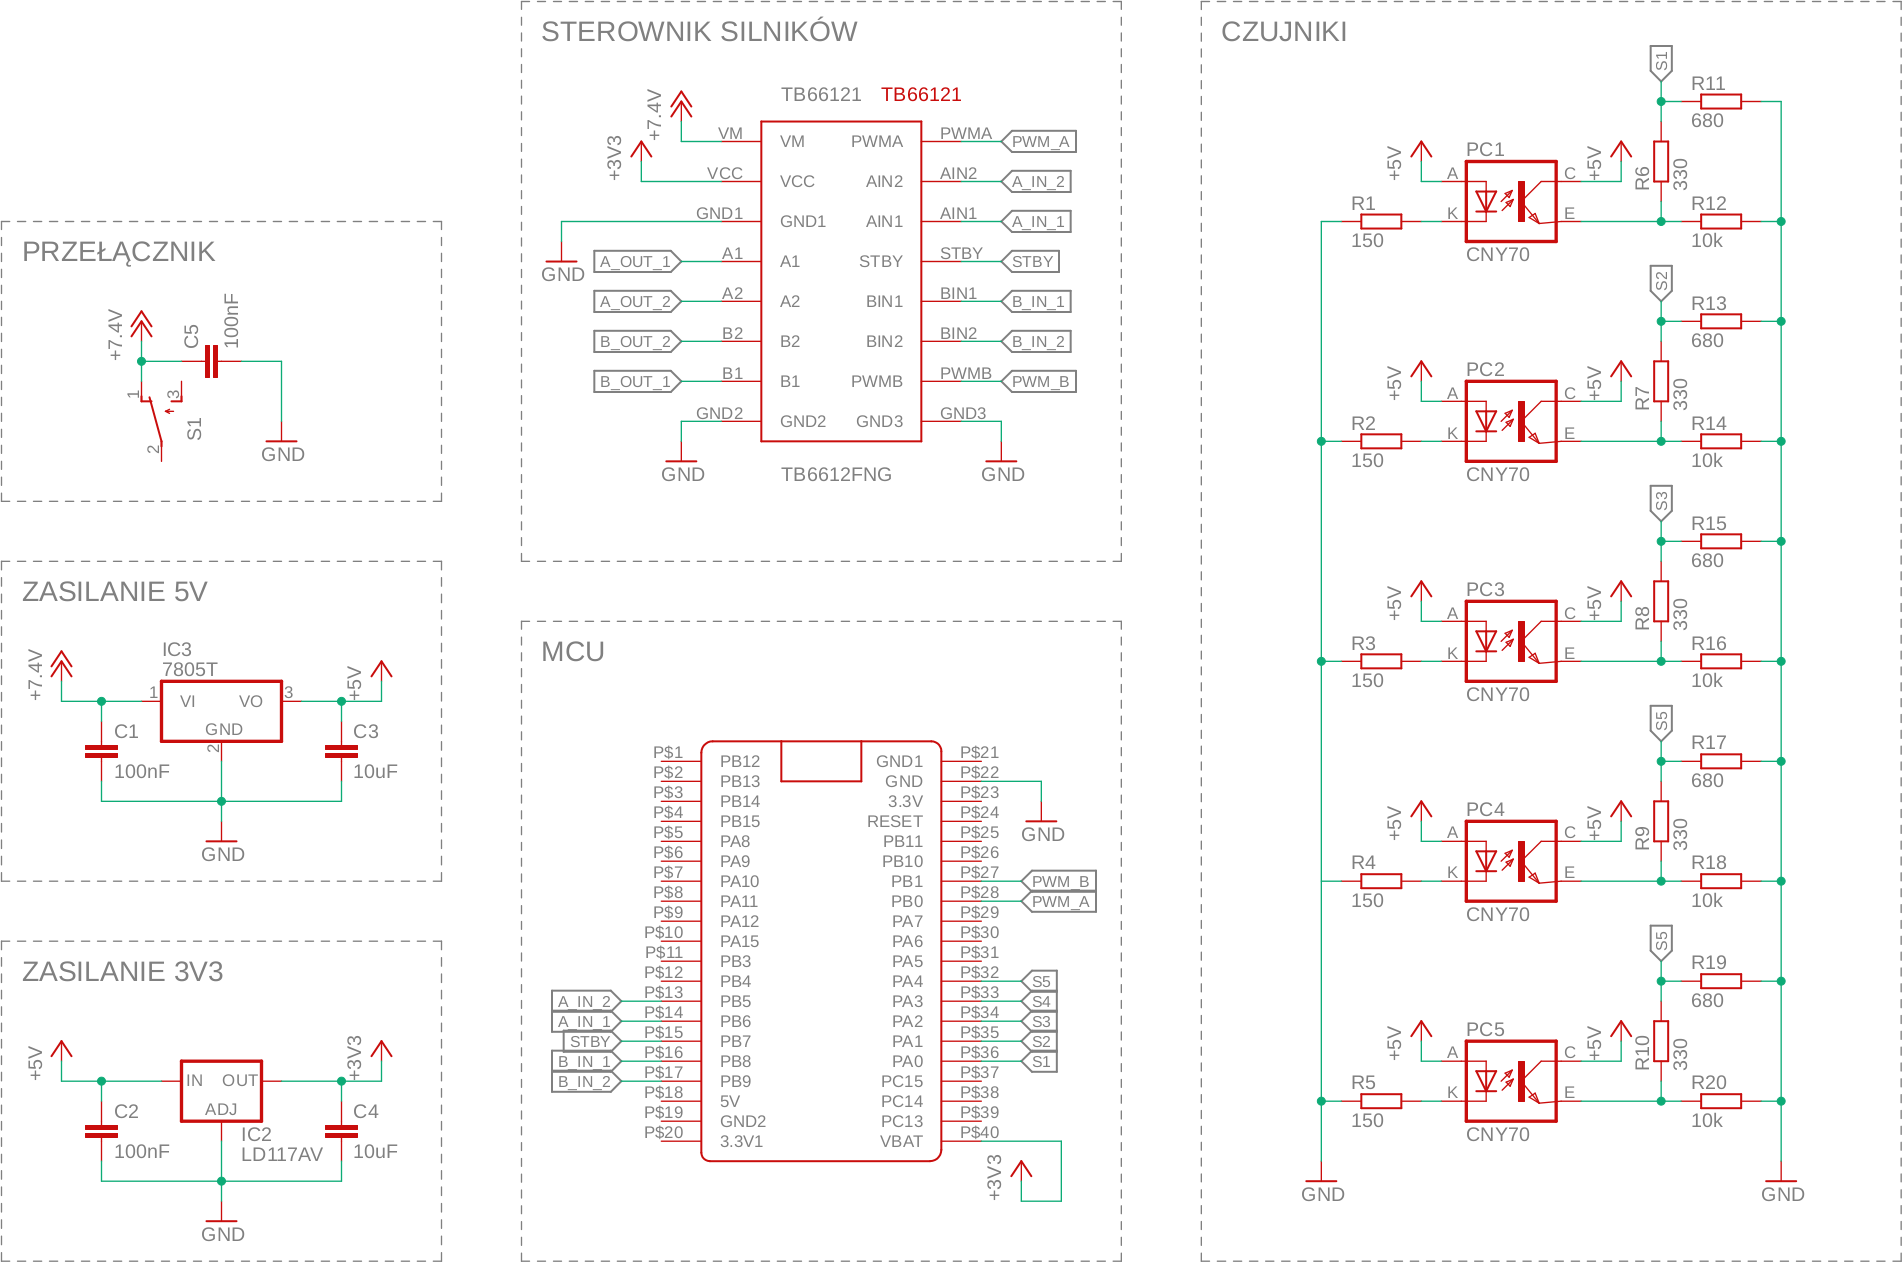
\includegraphics[width=1.4\textwidth, angle = 90]{schemat.png}
	\caption{Schemat układu}
	\label{fig:Schemat}
\end{figure}

\begin{table}[H]
	\centering
	\begin{tabular}{l|ll}
		\hline
		Part    & Value       & Device          \\ \hline
		C1      & 100nF       & C-EU025-024X044 \\ \hline
		C2      & 100nF       & C-EU025-024X044 \\ \hline
		C3      & 10uF        & C-EU025-024X044 \\ \hline
		C4      & 10uF        & C-EU025-024X044 \\ \hline
		C5      & 100nF       & C-EU025-024X044 \\ \hline
		IC2     & LD117V33     & LD117V33         \\ \hline
		IC3     & 7805         & LM7805           \\ \hline
		PC1     & CNY70       & CNY70           \\ \hline
		PC2     & CNY70       & CNY70           \\ \hline
		PC3     & CNY70       & CNY70           \\ \hline
		PC4     & CNY70       & CNY70           \\ \hline
		PC5     & CNY70       & CNY70           \\ \hline
		R1      & 150         & R-EU\_0204/5    \\ \hline
		R2      & 150         & R-EU\_0204/5    \\ \hline
		R3      & 150         & R-EU\_0204/5    \\ \hline
		R4      & 150         & R-EU\_0204/5    \\ \hline
		R5      & 150         & R-EU\_0204/5    \\ \hline
		R6      & 330         & R-EU\_0204/5    \\ \hline
		R7      & 330         & R-EU\_0204/5    \\ \hline
		R8      & 330         & R-EU\_0204/5    \\ \hline
		R9      & 330         & R-EU\_0204/5    \\ \hline
		R10     & 330         & R-EU\_0204/5    \\ \hline
		R11     & 680         & R-EU\_0204/5    \\ \hline
		R12     & 10k         & R-EU\_0204/5    \\ \hline
		R13     & 680         & R-EU\_0204/5    \\ \hline
		R14     & 10k         & R-EU\_0204/5    \\ \hline
		R15     & 680         & R-EU\_0204/5    \\ \hline
		R16     & 10k         & R-EU\_0204/5    \\ \hline
		R17     & 680         & R-EU\_0204/5    \\ \hline
		R18     & 10k         & R-EU\_0204/5    \\ \hline
		R19     & 680         & R-EU\_0204/5    \\ \hline
		R20     & 10k         & R-EU\_0204/5    \\ \hline
		S1      & TL32PO      & SWITCH          \\ \hline
		ST1     & STM32F103C8 & BLUE\_PILL      \\ \hline
		TB66121 & TB6612FNG   & TB6612FNG       \\ \hline
	\end{tabular}
	\caption{Zestawienie komponentów}
\end{table}
%Obecne we wszystkich dokumentach
\section{Podsumowanie}


\newpage
\addcontentsline{toc}{section}{Bibilografia}
\bibliography{bibliografia}
\bibliographystyle{plabbrv}


\end{document}
